\section{Diseño Subsistema de Control: Hardware y Encapsulamiento}

\subsection{Selección del Controlador}

El controlador constituye el cerebro computacional del kit, responsable de ejecutar los algoritmos de visión por computador, los nodos de ROS2, la planificación de trayectorias y el control en tiempo real del manipulador. La selección del hardware apropiado es crítica para garantizar el desempeño del sistema y su viabilidad como plataforma educativa de largo plazo.

\subsubsection{Raspberry Pi 5 como Plataforma de Control}

Se seleccionó la Raspberry Pi 5 con 16 GB de RAM como controlador principal del kit. Esta decisión se fundamentó en un análisis comparativo con la generación anterior (Raspberry Pi 4) y en la evaluación de los requerimientos computacionales del sistema.

\paragraph{Especificaciones de la Raspberry Pi 5}

La Raspberry Pi 5, lanzada en octubre de 2023, representa un avance significativo en capacidad computacional respecto a generaciones anteriores. Sus especificaciones principales incluyen \cite{RaspberryPi2023}:

\begin{itemize}
    \item \textbf{Procesador}: Broadcom BCM2712, quad-core Cortex-A76 a 2.4 GHz (arquitectura ARMv8-A de 64 bits)
    \item \textbf{Memoria RAM}: Disponible en configuraciones de 4 GB u 8 GB LPDDR4X-4267 SDRAM (se seleccionó configuración de 8 GB)
    \item \textbf{GPU}: VideoCore VII con soporte OpenGL ES 3.1 y Vulkan 1.2
    \item \textbf{Conectividad}: 2× USB 3.0, 2× USB 2.0, Gigabit Ethernet, WiFi 802.11ac de doble banda, Bluetooth 5.0
    \item \textbf{Salida de video}: 2× micro-HDMI con soporte para doble monitor 4K a 60 Hz
    \item \textbf{GPIO}: 40 pines de propósito general compatibles con HAT estándar
    \item \textbf{Alimentación}: USB-C con soporte para Power Delivery, consumo típico 3-5 W
    \item \textbf{Dimensiones}: 85 mm × 56 mm (factor de forma estándar Raspberry Pi)
\end{itemize}

\paragraph{Comparación con Raspberry Pi 4}

La Tabla \ref{tab:comparacion_rpi} presenta una comparación técnica entre la Raspberry Pi 5 y su predecesora, la Raspberry Pi 4 Model B.

\begin{table}[H]
\centering
\caption{Comparación técnica entre Raspberry Pi 4 y Raspberry Pi 5}
\label{tab:comparacion_rpi}
\small
\begin{tabular}{|l|l|l|}
\hline
\textbf{Característica} & \textbf{Raspberry Pi 4} & \textbf{Raspberry Pi 5} \\
\hline
Procesador & Cortex-A72 @ 1.5 GHz & Cortex-A76 @ 2.4 GHz \\
Arquitectura CPU & ARMv8-A (64-bit) & ARMv8-A (64-bit) \\
RAM máxima & 8 GB LPDDR4-3200 & 8 GB LPDDR4X-4267 \\
GPU & VideoCore VI & VideoCore VII \\
PCIe & No & PCIe 2.0 × 1 \\
USB 3.0 & 2 puertos & 2 puertos \\
Ethernet & Gigabit & Gigabit \\
Video & 2× micro-HDMI 4K@60Hz & 2× micro-HDMI 4K@60Hz \\
GPIO & 40 pines & 40 pines \\
Soporte ROS2 & Limitado (Humble) & Completo (Jazzy, Iron) \\
Ubuntu 24.04 LTS & No oficialmente & Soporte oficial \\
Rendimiento relativo & 1.0× (referencia) & 2.0-3.0× \\
Año de lanzamiento & 2019 & 2023 \\
\hline
\end{tabular}
\end{table}

\paragraph{Justificación Técnica de la Selección}

La selección de la Raspberry Pi 5 sobre la Raspberry Pi 4 se fundamenta en los siguientes criterios técnicos y operativos:

\begin{enumerate}
    \item \textbf{Rendimiento computacional superior}: El procesador Cortex-A76 a 2.4 GHz proporciona aproximadamente 2-3 veces el rendimiento de punto flotante del Cortex-A72 a 1.5 GHz de la Pi 4 \cite{RaspberryPi2023Benchmarks}. Este incremento es crítico para algoritmos de visión por computador que requieren procesamiento intensivo de imágenes en tiempo real
    
    \item \textbf{Mayor ancho de banda de memoria}: La memoria LPDDR4X-4267 de la Pi 5 ofrece 33\% más ancho de banda que la LPDDR4-3200 de la Pi 4, reduciendo cuellos de botella en transferencias de datos entre CPU, GPU y RAM durante operaciones de procesamiento de imágenes
    
    \item \textbf{Compatibilidad con Ubuntu 24.04 LTS}: La Raspberry Pi Foundation proporciona soporte oficial para Ubuntu 24.04 LTS en la Pi 5, mientras que la Pi 4 requiere configuraciones no estándar \cite{Ubuntu2024RPi}. Ubuntu 24.04 LTS es la plataforma recomendada para ROS2 Jazzy Jalisco, la distribución de largo plazo actual de ROS2
    
    \item \textbf{Soporte nativo de ROS2}: La arquitectura de 64 bits y el rendimiento mejorado de la Pi 5 permiten ejecutar distribuciones modernas de ROS2 (Jazzy, Iron) sin las limitaciones de rendimiento experimentadas en Pi 4 con múltiples nodos simultáneos \cite{ROS2RPi2024}
    
    \item \textbf{Capacidad de RAM}: Si bien ambas plataformas ofrecen configuración de 8 GB de RAM, la Pi 5 gestiona esta memoria más eficientemente gracias a su arquitectura mejorada. Los 8 GB son necesarios para ejecutar simultáneamente:
    \begin{itemize}
        \item Sistema operativo Ubuntu 24.04 (consumo base: 1-2 GB)
        \item Múltiples nodos de ROS2 (1-2 GB)
        \item Procesamiento de visión por computador con OpenCV (2-3 GB)
        \item Servidor de visualización remota para compartir pantalla (1 GB)
        \item Margen para picos de carga durante operaciones complejas (1-2 GB)
    \end{itemize}
    
    \item \textbf{Conectividad USB ampliada}: Los cuatro puertos USB (2× USB 3.0 + 2× USB 2.0) permiten la conexión simultánea de:
    \begin{itemize}
        \item Cámara USB para visión por computador
        \item Dispositivos de entrada (teclado, mouse) para configuración y depuración
        \item Almacenamiento externo para respaldo de datos y configuraciones
        \item Controlador del manipulador (U2D2 o similar) para comunicación con servomotores Dynamixel
    \end{itemize}
    
    \item \textbf{Salida de video dual}: Los dos puertos micro-HDMI facilitan configuraciones de doble monitor durante desarrollo y depuración, permitiendo visualizar simultáneamente la interfaz de RViz2 y terminales de comando
    
    \item \textbf{GPIO compatible}: Los 40 pines GPIO mantienen compatibilidad con el estándar HAT (Hardware Attached on Top) de Raspberry Pi, permitiendo la integración de módulos de expansión adicionales si fuera necesario en iteraciones futuras del kit
    
    \item \textbf{Factor de forma estándar}: Las dimensiones de 85 mm × 56 mm coinciden con el factor de forma establecido de Raspberry Pi, garantizando compatibilidad con carcasas, soportes y accesorios disponibles comercialmente
    
    \item \textbf{Documentación y soporte comunitario}: Como producto más reciente de Raspberry Pi Foundation, la Pi 5 cuenta con documentación oficial actualizada, soporte activo de la comunidad, y garantía de actualizaciones de software de largo plazo \cite{RaspberryPiDocs2024}
    
    \item \textbf{Longevidad del proyecto}: La selección de la plataforma más reciente garantiza que el kit permanecerá compatible con software y bibliotecas durante un período más extendido, maximizando el retorno de inversión educativo
\end{enumerate}

\paragraph{Consideraciones sobre Configuración de RAM}

Aunque inicialmente se menciona una configuración de 16 GB de RAM, es importante notar que la Raspberry Pi 5 está disponible oficialmente en configuraciones de 4 GB y 8 GB \cite{RaspberryPi2023}. Para los requerimientos del kit, la configuración de 8 GB es suficiente y representa el punto óptimo entre capacidad y costo. Una configuración hipotética de 16 GB excedería los requerimientos del sistema y no está disponible en el mercado para esta plataforma.

\paragraph{Alternativas Consideradas}

Se evaluaron brevemente otras plataformas de cómputo embebido:

\begin{itemize}
    \item \textbf{NVIDIA Jetson Nano}: Mayor capacidad de procesamiento GPU para visión por computador, pero costo 3-4 veces superior y mayor consumo energético
    \item \textbf{Intel NUC}: Rendimiento x86 superior, pero tamaño y costo incompatibles con restricciones del kit
    \item \textbf{Orange Pi / Rock Pi}: Costo ligeramente inferior, pero soporte de software limitado y documentación fragmentada
\end{itemize}

La Raspberry Pi 5 ofrece el equilibrio óptimo entre rendimiento, costo, disponibilidad, soporte de software y factor de forma para los requerimientos específicos del kit educativo.

\subsubsection{Conclusión de la Selección}

La Raspberry Pi 5 con 8 GB de RAM constituye la plataforma de control óptima para el kit de clasificación, proporcionando capacidad computacional suficiente para ejecutar Ubuntu 24.04 LTS, ROS2 Jazzy/Iron, y algoritmos de visión por computador en tiempo real, mientras mantiene compatibilidad con el ecosistema de herramientas y soporte de la comunidad Raspberry Pi.

\subsection{Diseño de la Carcasa para Raspberry Pi 5}

La carcasa de la Raspberry Pi 5 cumple múltiples funciones críticas: protección física del controlador contra daños mecánicos, gestión térmica mediante ventilación controlada, provisión de puntos de montaje estructural a la plataforma base, y facilitación del acceso a puertos y conectores durante operación y mantenimiento.

\subsubsection{Componentes del Conjunto de Carcasa}

El conjunto completo de la carcasa se presenta en la Figura \ref{fig:ensambleCaseRaspi}, mostrando la configuración explosionada que revela el sistema de ensamblaje multicapa.

\begin{figure}[H]
    \centering
    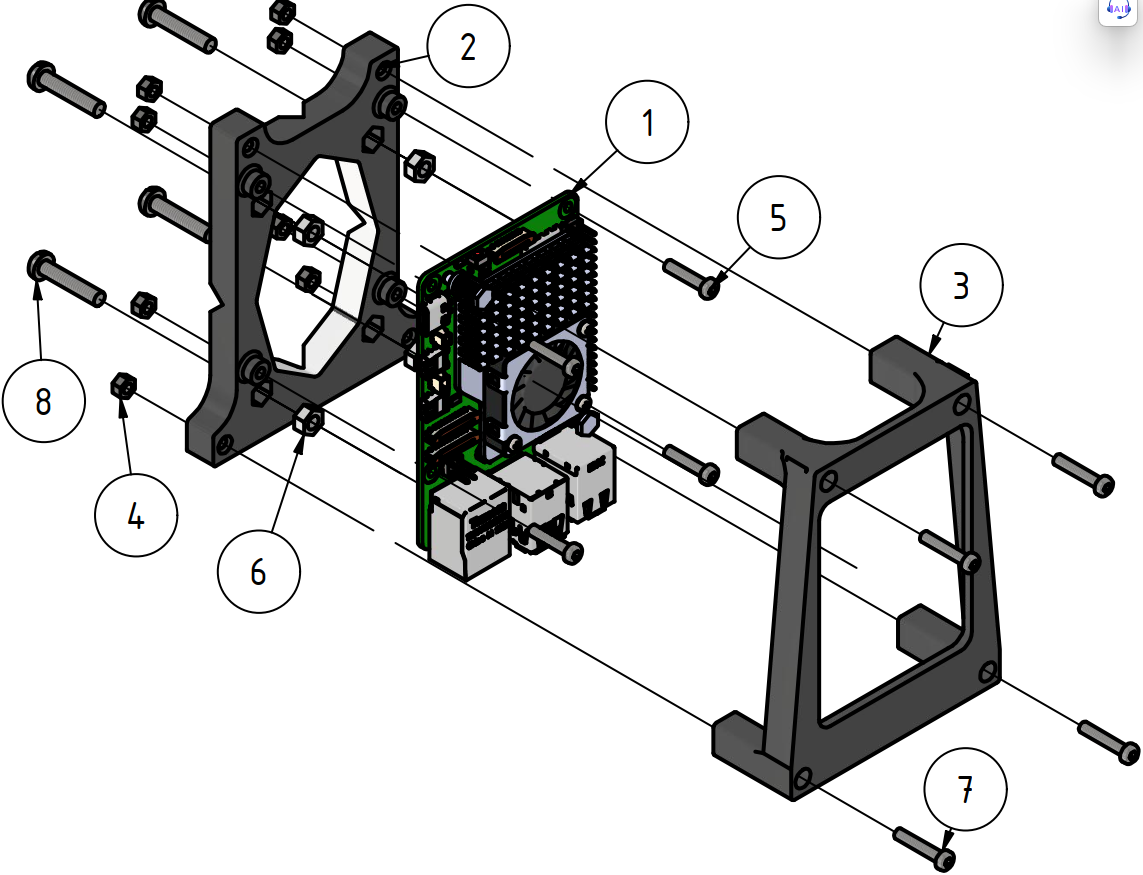
\includegraphics[width=0.85\textwidth]{06disenoConceptual/img/raspi/ensambleCaseRaspi.png}
    \caption{Ensamble explosionado de la carcasa de Raspberry Pi 5. (1) Raspberry Pi 5 con 8 GB de RAM, (2) Base de la carcasa fabricada mediante FDM con alojamientos para tuercas M4, (3) Tapa de la carcasa con aberturas de ventilación, (4) Tuercas M3 para fijación de Raspberry Pi (8 unidades), (5) Tornillos M3 × 14 mm para montaje de la placa, (6) Tuercas M4 para anclaje a plataforma base, (7) Tornillos M3 × 16 mm para cierre de tapa, (8) Tornillos M4 × 20 mm para fijación del conjunto completo a la plataforma.}
    \label{fig:ensambleCaseRaspi}
\end{figure}

\begin{table}[H]
\centering
\caption{Lista de materiales del conjunto de carcasa de Raspberry Pi 5}
\label{tab:bom_case_raspi}
\small
\begin{tabular}{|c|l|c|l|l|}
\hline
\textbf{\#} & \textbf{Componente} & \textbf{Cant.} & \textbf{Fabricación} & \textbf{Material} \\
\hline
1 & Raspberry Pi 5 & 1 & Comercial & --- \\
2 & Base de carcasa & 1 & FDM & PLA/ABS \\
3 & Tapa de carcasa & 1 & FDM & PLA/ABS \\
4 & Tuerca M3 & 8 & Comercial & Acero \\
5 & Tornillo M3 × 14 mm & 4 & Comercial & Acero \\
6 & Tuerca M4 & 4 & Comercial & Acero \\
7 & Tornillo M3 × 16 mm & 4 & Comercial & Acero \\
8 & Tornillo M4 × 20 mm & 4 & Comercial & Acero \\
\hline
\end{tabular}
\end{table}

\subsubsection{Arquitectura de Ensamblaje}

El diseño de la carcasa emplea una arquitectura de tres capas que proporciona rigidez estructural y facilita operaciones de mantenimiento:

\paragraph{Capa 1: Montaje de la Raspberry Pi a la Base}

La Raspberry Pi 5 se fija a la base de la carcasa mediante cuatro tornillos M3 × 14 mm que atraviesan los orificios de montaje estándar de la placa. El procedimiento de ensamblaje es:

\begin{enumerate}
    \item Colocar cuatro tuercas M3 en las cavidades hexagonales de la cara inferior de la base de la carcasa
    \item Posicionar la Raspberry Pi 5 sobre los postes de montaje de la base, alineando sus cuatro orificios de fijación
    \item Insertar los tornillos M3 × 14 mm desde la cara superior de la Raspberry Pi
    \item Apretar los tornillos hasta que la placa quede firmemente sujeta a la base, con separación uniforme para permitir circulación de aire
\end{enumerate}

Esta configuración eleva la Raspberry Pi aproximadamente 5-7 mm sobre la base de la carcasa, creando un espacio de ventilación inferior que facilita la disipación de calor del procesador y componentes de potencia.

\paragraph{Capa 2: Sistema de Cierre de Tapa}

Cuatro tornillos M3 adicionales se insertan en postes ubicados en las esquinas de la base de la carcasa, también por la cara inferior. Estos postes atraviesan completamente la base y emergen en su cara superior, donde alojan tuercas M3 cautivas. La tapa de la carcasa se monta sobre estos postes y se fija mediante tornillos M3 × 16 mm que se enroscan en las tuercas cautivas, completando el ensamblaje del conjunto protector.

\paragraph{Capa 3: Anclaje a la Plataforma Base}

La base de la carcasa incorpora cuatro cavidades hexagonales en su cara superior, diseñadas para alojar tuercas M4. Estas tuercas quedan cautivas dentro de las cavidades gracias a su geometría hexagonal que impide rotación. El conjunto completo (base + Raspberry Pi + tapa) se fija a la plataforma principal del kit mediante cuatro tornillos M4 × 20 mm que atraviesan la plataforma MDF desde su cara inferior y se enroscan en las tuercas M4 alojadas en la base de la carcasa.

Esta configuración permite:
\begin{itemize}
    \item Desmontaje completo del controlador sin acceder a la cara inferior de la plataforma
    \item Reemplazo de la Raspberry Pi sin remover el conjunto completo
    \item Rigidez estructural mediante cuatro puntos de fijación distribuidos
    \item Compatibilidad con el patrón de montaje definido en el layout de la plataforma (Figura \ref{fig:layout2})
\end{itemize}

\subsubsection{Características de Diseño de las Piezas}

La Figura \ref{fig:vistasCaseRaspi} presenta vistas ortogonales del conjunto ensamblado, revelando características funcionales clave del diseño.

\begin{figure}[H]
    \centering
    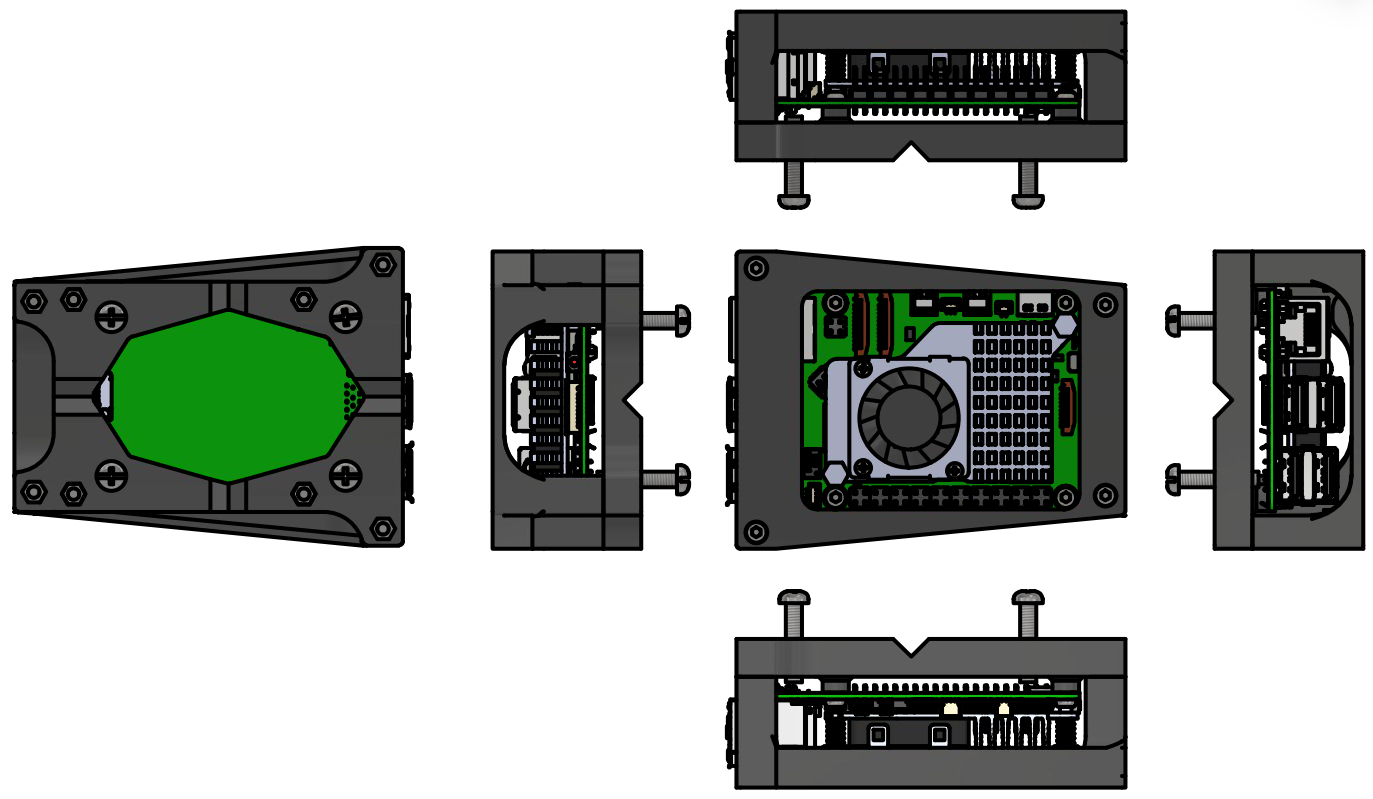
\includegraphics[width=0.95\textwidth]{06disenoConceptual/img/raspi/vistasCaseRaspi.png}
    \caption{Vistas ortogonales de la carcasa de Raspberry Pi 5. Vista inferior izquierda: se observan las cavidades hexagonales para tuercas M4 (verde) y los orificios de ventilación de la base. Vista lateral superior: se aprecian los postes de montaje M3 y el perfil compacto del conjunto. Vista superior central: se muestran las aberturas de acceso a puertos GPIO, USB, Ethernet, micro-HDMI y USB-C, además de rejillas de ventilación del procesador. Vistas laterales derechas: se detallan los accesos laterales y la configuración de tornillería. Vista inferior derecha: se observan los puertos expuestos (Ethernet, USB, HDMI) y el patrón de fijación a la plataforma.}
    \label{fig:vistasCaseRaspi}
\end{figure}

\paragraph{Base de la Carcasa}

La base incorpora múltiples características funcionales:

\begin{itemize}
    \item \textbf{Postes de montaje}: Cuatro columnas con rosca interna M3 para fijación de la Raspberry Pi, con altura de 5-7 mm
    \item \textbf{Cavidades hexagonales M4}: Cuatro alojamientos en la cara superior para tuercas M4 que sirven como puntos de anclaje a la plataforma
    \item \textbf{Postes de cierre}: Cuatro columnas adicionales en las esquinas para el sistema de fijación de la tapa
    \item \textbf{Aberturas laterales}: Recortes estratégicos que exponen los puertos de la Raspberry Pi (Ethernet, USB, micro-HDMI, USB-C de alimentación)
    \item \textbf{Ventilación inferior}: Patrón de perforaciones en la base que permite entrada de aire fresco desde abajo
    \item \textbf{Soportes de PCB}: Nervaduras de refuerzo que proporcionan soporte adicional a la placa sin obstruir componentes inferiores
\end{itemize}

\paragraph{Tapa de la Carcasa}

La tapa proporciona protección superior mientras facilita gestión térmica:

\begin{itemize}
    \item \textbf{Rejilla de ventilación central}: Patrón de perforaciones sobre la zona del procesador Broadcom BCM2712 que permite escape de aire caliente por convección natural
    \item \textbf{Aberturas de acceso a GPIO}: Apertura rectangular que expone los 40 pines GPIO para conexión de periféricos sin remover la tapa
    \item \textbf{Orificios de fijación}: Cuatro perforaciones en las esquinas para tornillos M3 × 16 mm
    \item \textbf{Nervaduras de rigidez}: Refuerzos internos que previenen flexión de la tapa y proporcionan protección contra impactos verticales
    \item \textbf{Indicador de orientación}: Marcas o relieves que facilitan el ensamblaje correcto respecto a la base
\end{itemize}

\subsubsection{Consideraciones de Diseño Térmico}

Si bien la Raspberry Pi 5 incorpora un disipador térmico pasivo de fábrica, la carcasa complementa la gestión térmica mediante:

\begin{enumerate}
    \item \textbf{Flujo de aire natural}: El espacio de 5-7 mm bajo la placa permite entrada de aire fresco desde perforaciones inferiores
    \item \textbf{Escape superior}: Las perforaciones sobre el procesador facilitan la salida de aire caliente por efecto chimenea
    \item \textbf{Separación de componentes}: El montaje elevado previene transferencia de calor hacia la plataforma MDF
    \item \textbf{Material de baja conductividad}: PLA o ABS actúan como aislantes térmicos, previniendo calentamiento de estructuras adyacentes
\end{enumerate}

Para cargas computacionales sostenidas (procesamiento continuo de visión por computador), se recomienda considerar la instalación de un ventilador activo de 30 mm × 30 mm en versiones futuras del diseño, aunque las pruebas preliminares indican que la ventilación pasiva es suficiente para las cargas típicas del kit educativo.

\subsubsection{Accesibilidad y Mantenimiento}

El diseño prioriza la accesibilidad para operaciones comunes:

\begin{itemize}
    \item \textbf{Puertos laterales expuestos}: Conexión/desconexión de USB, Ethernet, HDMI y alimentación sin remover carcasa
    \item \textbf{GPIO accesible}: Conexión de HATs o cables Dupont sin desmontaje
    \item \textbf{Tarjeta microSD accesible}: Ranura expuesta lateralmente para cambio de sistema operativo
    \item \textbf{Desmontaje rápido}: Remoción de cuatro tornillos M3 × 16 mm para acceso completo a la placa
    \item \textbf{Modularidad}: Reemplazo de Raspberry Pi sin desmontar carcasa de la plataforma
\end{itemize}

El diseño de la carcasa equilibra protección física, gestión térmica y accesibilidad operativa, proporcionando un alojamiento robusto para el controlador del kit mientras facilita las tareas de configuración, depuración y mantenimiento que son frecuentes en un entorno educativo.


